% !TEX program = xelatex
% Consolidated final report — Phases 1, 2 and 3
% Build: xelatex final_report.tex (run twice)
\documentclass[11pt,a4paper]{article}

\usepackage[a4paper,margin=2.2cm]{geometry}
\usepackage{fontspec}
\usepackage{graphicx}
\usepackage{booktabs}
\usepackage{array}
\usepackage{multirow}
\usepackage{amsmath}
\usepackage{amssymb}
\usepackage{float}
\usepackage{enumitem}
\usepackage{titlesec}
\usepackage{xcolor}
\usepackage{fancyhdr}
\usepackage[font=small,labelfont=bf]{caption}
\usepackage{microtype}
\usepackage[hidelinks]{hyperref}
\usepackage{xurl}

% ---------- Fonts ----------
\setmainfont{Georgia}
\setsansfont{Calibri}
\newfontfamily\devanagarafont{Nirmala UI}[Script=Devanagari]
\newfontfamily\bengalifont{Nirmala UI}[Script=Bengali]
\newcommand{\dv}[1]{{\devanagarafont #1}}
\newcommand{\as}[1]{{\bengalifont #1}}

% ---------- Headings ----------
\definecolor{headblue}{RGB}{28,60,90}
\titleformat{\section}{\normalfont\sffamily\bfseries\large\color{headblue}}{\thesection}{0.6em}{}
\titleformat{\subsection}{\normalfont\sffamily\bfseries\normalsize}{\thesubsection}{0.6em}{}
\titlespacing*{\section}{0pt}{12pt plus 2pt}{6pt}
\titlespacing*{\subsection}{0pt}{9pt plus 2pt}{4pt}

% ---------- Misc ----------
\setlist{itemsep=1pt,topsep=3pt,parsep=0pt}
\graphicspath{{figures/}}
\captionsetup{skip=4pt}
\pagestyle{fancy}
\fancyhf{}
\fancyhead[L]{\footnotesize\itshape Language Models and Agents (Monsoon 2026)}
\fancyhead[R]{\footnotesize\thepage}
\renewcommand{\headrulewidth}{0.3pt}
\linespread{1.03}
\setlength{\parskip}{2pt}
\setlength{\emergencystretch}{3em}

\begin{document}

% ============================ TITLE ============================
\begin{center}
{\sffamily\bfseries\Large Monolingual Language Models for Hindi and Assamese:\\[2pt]
Data, Pretraining, and Symbolic Reasoning}\\[8pt]
{\normalsize Consolidated Final Report (Phases 1, 2 and 3)}\\[8pt]
Shubhadeep Mandal \; (Roll No.\ 2025201056)\\
\small Branch \texttt{phase-3} \,\textbullet\, Language Models and Agents, Monsoon 2026\\[2pt]
\footnotesize Higher-resource model H: Hindi (Devanagari) \,\textbullet\, Lower-resource model L: Assamese (Eastern Nagari, \as{অসমীয়া})
\end{center}
\vspace{-2pt}

\noindent\textbf{Abstract.}
This report consolidates the whole project. In Phase~1 I built two strictly separate data pipelines and trained a 16{,}384-piece SentencePiece BPE tokenizer for each language; Hindi reached 723.32M cleaned tokens (20.55\% collected manually) and Assamese 528.50M (22.48\% manually). In Phase~2 I implemented and pretrained two $\sim$25M-parameter decoder-only transformers per language from scratch, a hand-written baseline (V1) and a modern variant (V2) with RoPE, SwiGLU and RMSNorm, on 500M tokens each. The modern model won everywhere: test perplexity 52.26 vs.\ 82.28 (Hindi) and 80.93 vs.\ 120.54 (Assamese). In Phase~3 I generated a leak-proof synthetic relational-reasoning suite and fine-tuned eight models (both architectures $\times$ direct SFT vs.\ chain-of-thought). Chain-of-thought training clearly improves output quality (answer F1, character similarity, decomposed step score), while direct SFT keeps a small edge in strict exact match. A four-layer attention study shows that fine-tuning sharpens entity-focused heads and increases the distance between query and premise tokens. The final section answers the four comparison questions from the assignment brief.

\vspace{2pt}
\noindent\footnotesize Artifacts. Phase~1 corpora and tokenizers: \url{https://www.kaggle.com/datasets/shubhadeepmandal/lma-hindi-artifacts} and \url{https://www.kaggle.com/datasets/shubhadeepmandal/lma-assamese-artifact}; Phase~2 checkpoints: \url{https://www.kaggle.com/datasets/shubhadeepmandal/lma-phase2-artifacts}; Phase~3 checkpoints: \url{https://www.kaggle.com/datasets/shubhadeepmandal/lma-phase3-artifact}. Code: \texttt{github.com/CL3-410/individual-project-Seronic2001} (branch \texttt{phase-3}).

% ============================ OVERVIEW ============================
\section{Project overview}

\begin{table}[H]
\centering\small
\begin{tabular}{@{}p{0.30\textwidth}p{0.30\textwidth}p{0.30\textwidth}@{}}
\toprule
\textbf{Phase 1, Data \& tokenizers} & \textbf{Phase 2, Pretraining} & \textbf{Phase 3, Reasoning} \\
\midrule
Custom multi-threaded crawlers + textbook OCR; NFKC normalisation, script filtering, SHA-256 and MinHash dedup; 98/1/1 splits; four tokenizer candidates compared per language. &
Two architectures per language, both 8 layers, $d_{\text{model}}{=}384$: V1 (learned positions, GELU, LayerNorm) and V2 (RoPE, SwiGLU, RMSNorm). 500M tokens, AdamW + cosine, fp16. &
Synthetic comparative-reasoning suite (6 paradigms) with disjoint train/test entity pools; 8 fine-tuned models; 5-tier metric suite; pre- vs.\ post-finetune attention analysis. \\
\bottomrule
\end{tabular}
\end{table}

\noindent The two languages share no data, code paths, tokenizers or parameters; every component exists twice, once per language. All models were trained on Kaggle GPUs (P100/T4) within the free tier.

% ============================ PHASE 1 ============================
\section{Phase 1: corpora and tokenizers}

\subsection{Collecting and cleaning the data}

For Hindi, large web corpora (Sangraha, OSCAR, Wikipedia) already exist, so the manual share came from my own crawlers over literature archives (Gadyakosh, Kavitakosh), news portals, and NCERT textbook PDFs (digital extraction plus Tesseract OCR). Assamese was harder. Public Assamese text is thin and often mislabelled as Bengali, so a larger fraction of the corpus came from targeted crawls over regional news portals (Asomiya Pratidin, NENow, Niyomiya Barta, EastMojo/ETV Bharat, Dainik Agradoot), literary archives, and OCR over 1{,}840 SCERT/SEBA/NCERT textbooks.

All documents from all sources passed through the same deterministic pipeline (\texttt{clean.py}):
\begin{enumerate}
  \item \textbf{Unicode canonicalisation}: NFKC, zero-width character control (ZWJ/ZWNJ), nukta healing (e.g.\ \dv{क + ़ -> क़}), and repair of ASCII periods/pipes into the proper purna viram \dv{।};
  \item \textbf{script-ratio filter}: discard any document with under 80\% of its characters in the target Unicode block (this removes English boilerplate and Bengali--Assamese confusion);
  \item \textbf{deduplication}: exact SHA-256 hashes plus MinHash/LSH near-duplicate removal at a 0.6 Jaccard threshold (1{,}859{,}349 duplicates dropped in Hindi; 114{,}290 in Assamese);
  \item \textbf{splitting}: deterministic 98/1/1 train/val/test split (seed 1337), then streamed into flat uint16 token binaries.
\end{enumerate}

\begin{table}[H]
\centering\small
\caption{Corpus summary (rubric: $\sim$500M tokens, $\geq$20\% manually collected; both languages comply).}
\begin{tabular}{@{}lrr@{}}
\toprule
 & \textbf{Hindi (H)} & \textbf{Assamese (L)} \\
\midrule
Total clean tokens & \textbf{723,321,981} & \textbf{528,500,000} \\
Manually collected & 148,676,877 (20.55\%) & 118,800,000 (22.48\%) \\
Downloaded corpora & 574,645,104 (79.45\%) & 409,700,000 (77.52\%) \\
Dedup removed & 1,859,349 docs & 114,290 docs \\
\bottomrule
\end{tabular}
\end{table}

\begin{figure}[H]
\centering
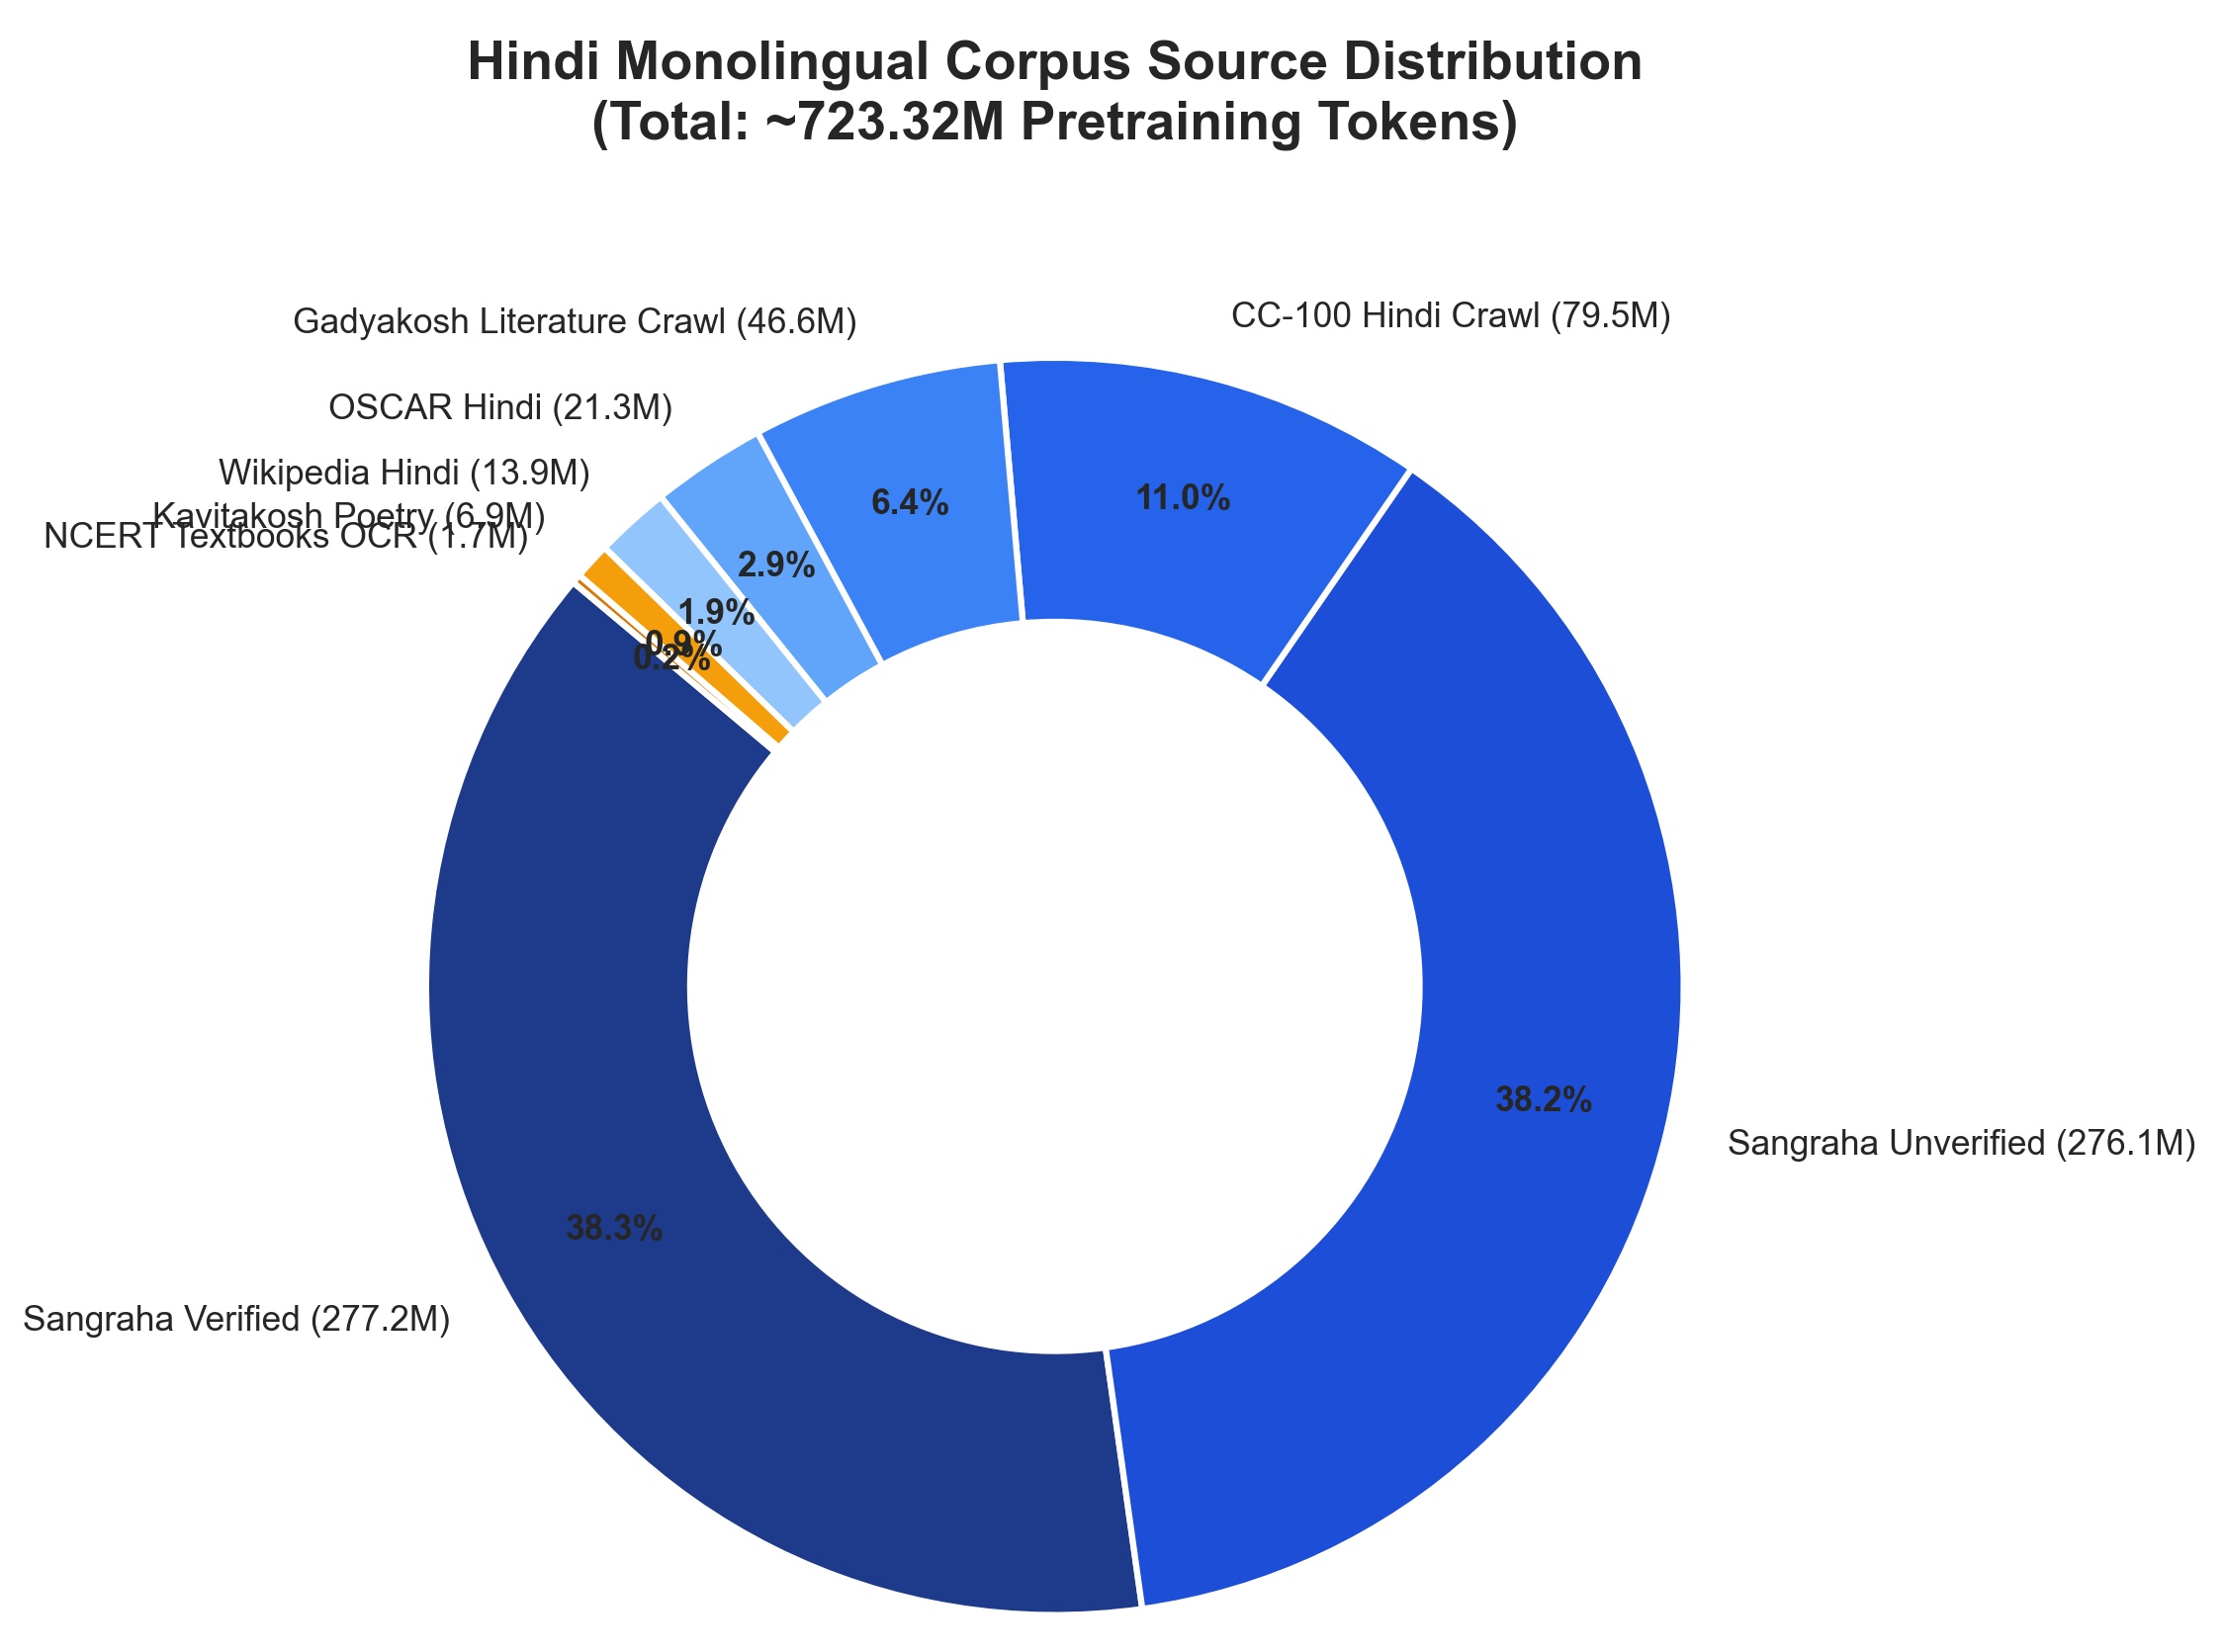
\includegraphics[width=0.48\textwidth]{corpus_distribution_hindi_cropped.png}\hfill
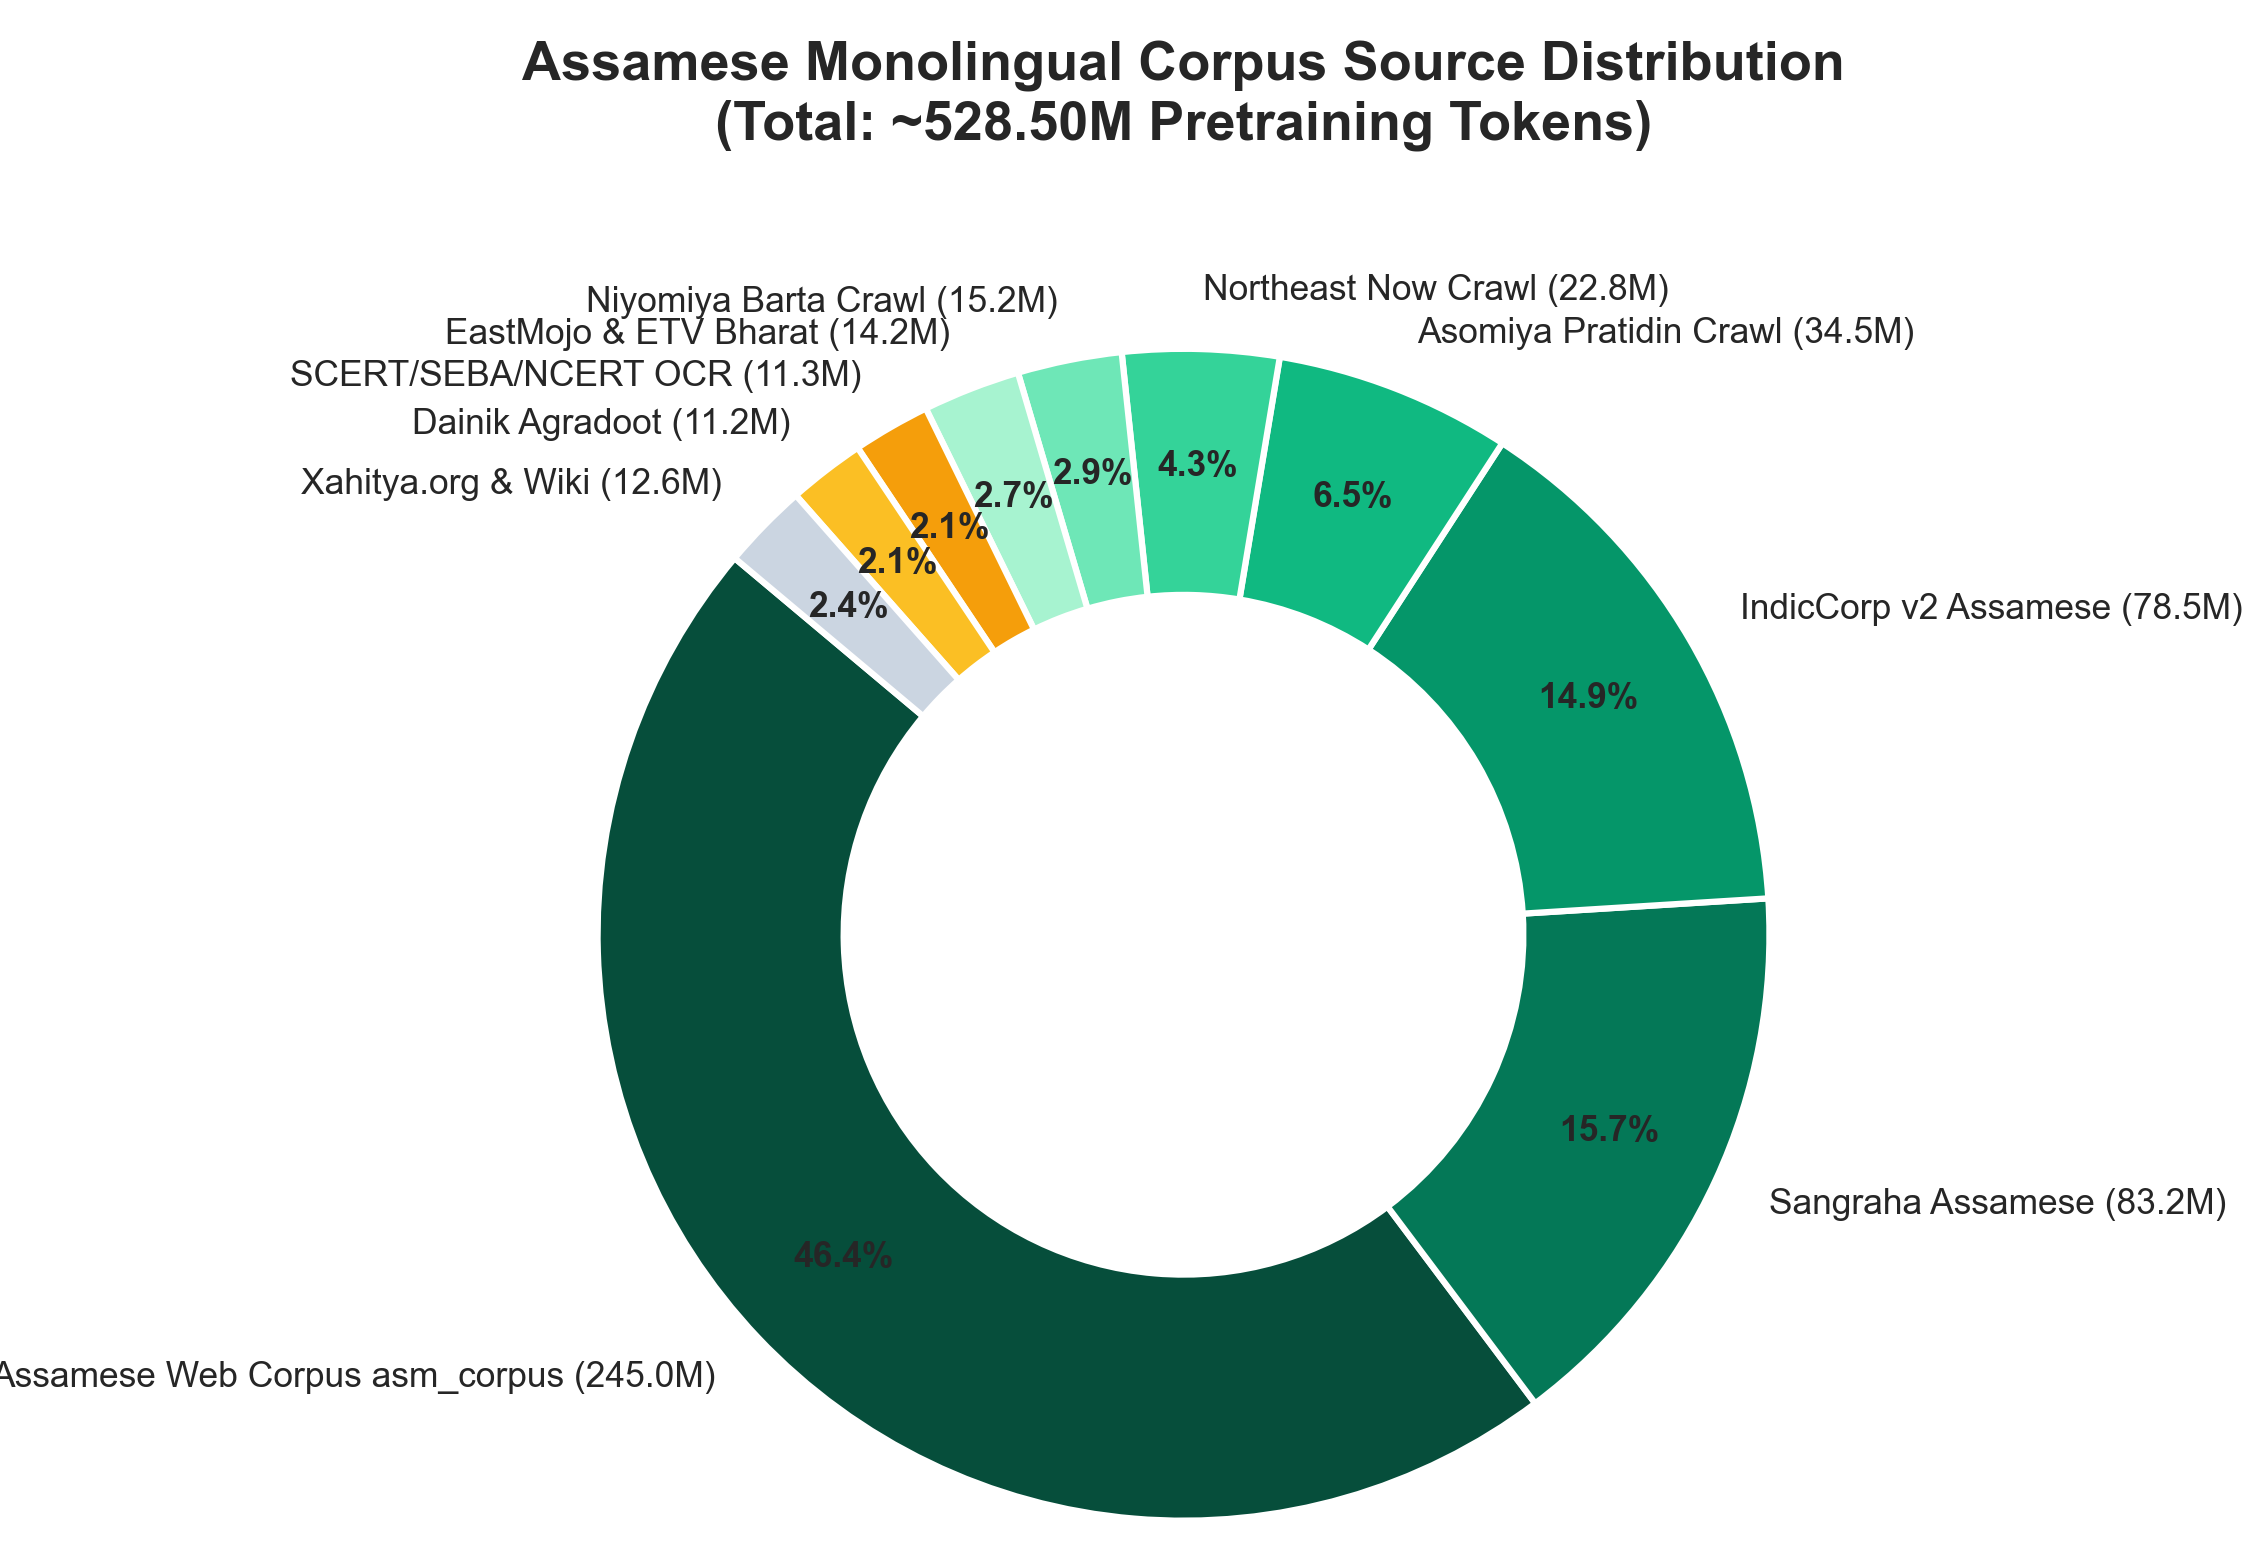
\includegraphics[width=0.48\textwidth]{corpus_distribution_assamese_cropped.png}
\caption{Corpus composition by source. Left: Hindi (723.32M tokens, 20.55\% manual). Right: Assamese (528.50M tokens, 22.48\% manual).}
\end{figure}

\subsection{Choosing a tokenizer}

Four candidates per language (BPE/Unigram $\times$ 16K/32K) were trained with SentencePiece (\texttt{character\_coverage=1.0}, \texttt{byte\_fallback=true}, digits split, scripts not merged) and scored on held-out text.

\begin{table}[H]
\centering\small
\caption{Fertility (tokens per word) of the four candidates; unk rate was 0.0000\% for all.}
\begin{tabular}{@{}lcccc@{}}
\toprule
 & BPE 16K & BPE 32K & Unigram 16K & Unigram 32K \\
\midrule
Hindi & \textbf{1.1858} & 1.1252 & 1.2728 & 1.2065 \\
Assamese & \textbf{1.4426} & 1.3130 & 1.4091 & 1.2978 \\
\bottomrule
\end{tabular}
\end{table}

The 32K vocabularies compress slightly better, but at $d_{\text{model}}{=}384$ a 32K embedding table costs $32{,}768 \times 384 = 12.58$M parameters, half the model budget, while 16K costs 6.29M. Choosing 16K freed enough room to grow from 6 to 8 transformer layers, and the fertility penalty is small (Hindi $1.19$ vs $1.13$; Assamese $1.44$ vs $1.31$). Both chosen 16K BPE tokenizers reconstruct held-out text exactly (100\% roundtrip) and never emit \texttt{<unk>} thanks to byte fallback.

\begin{figure}[H]
\centering
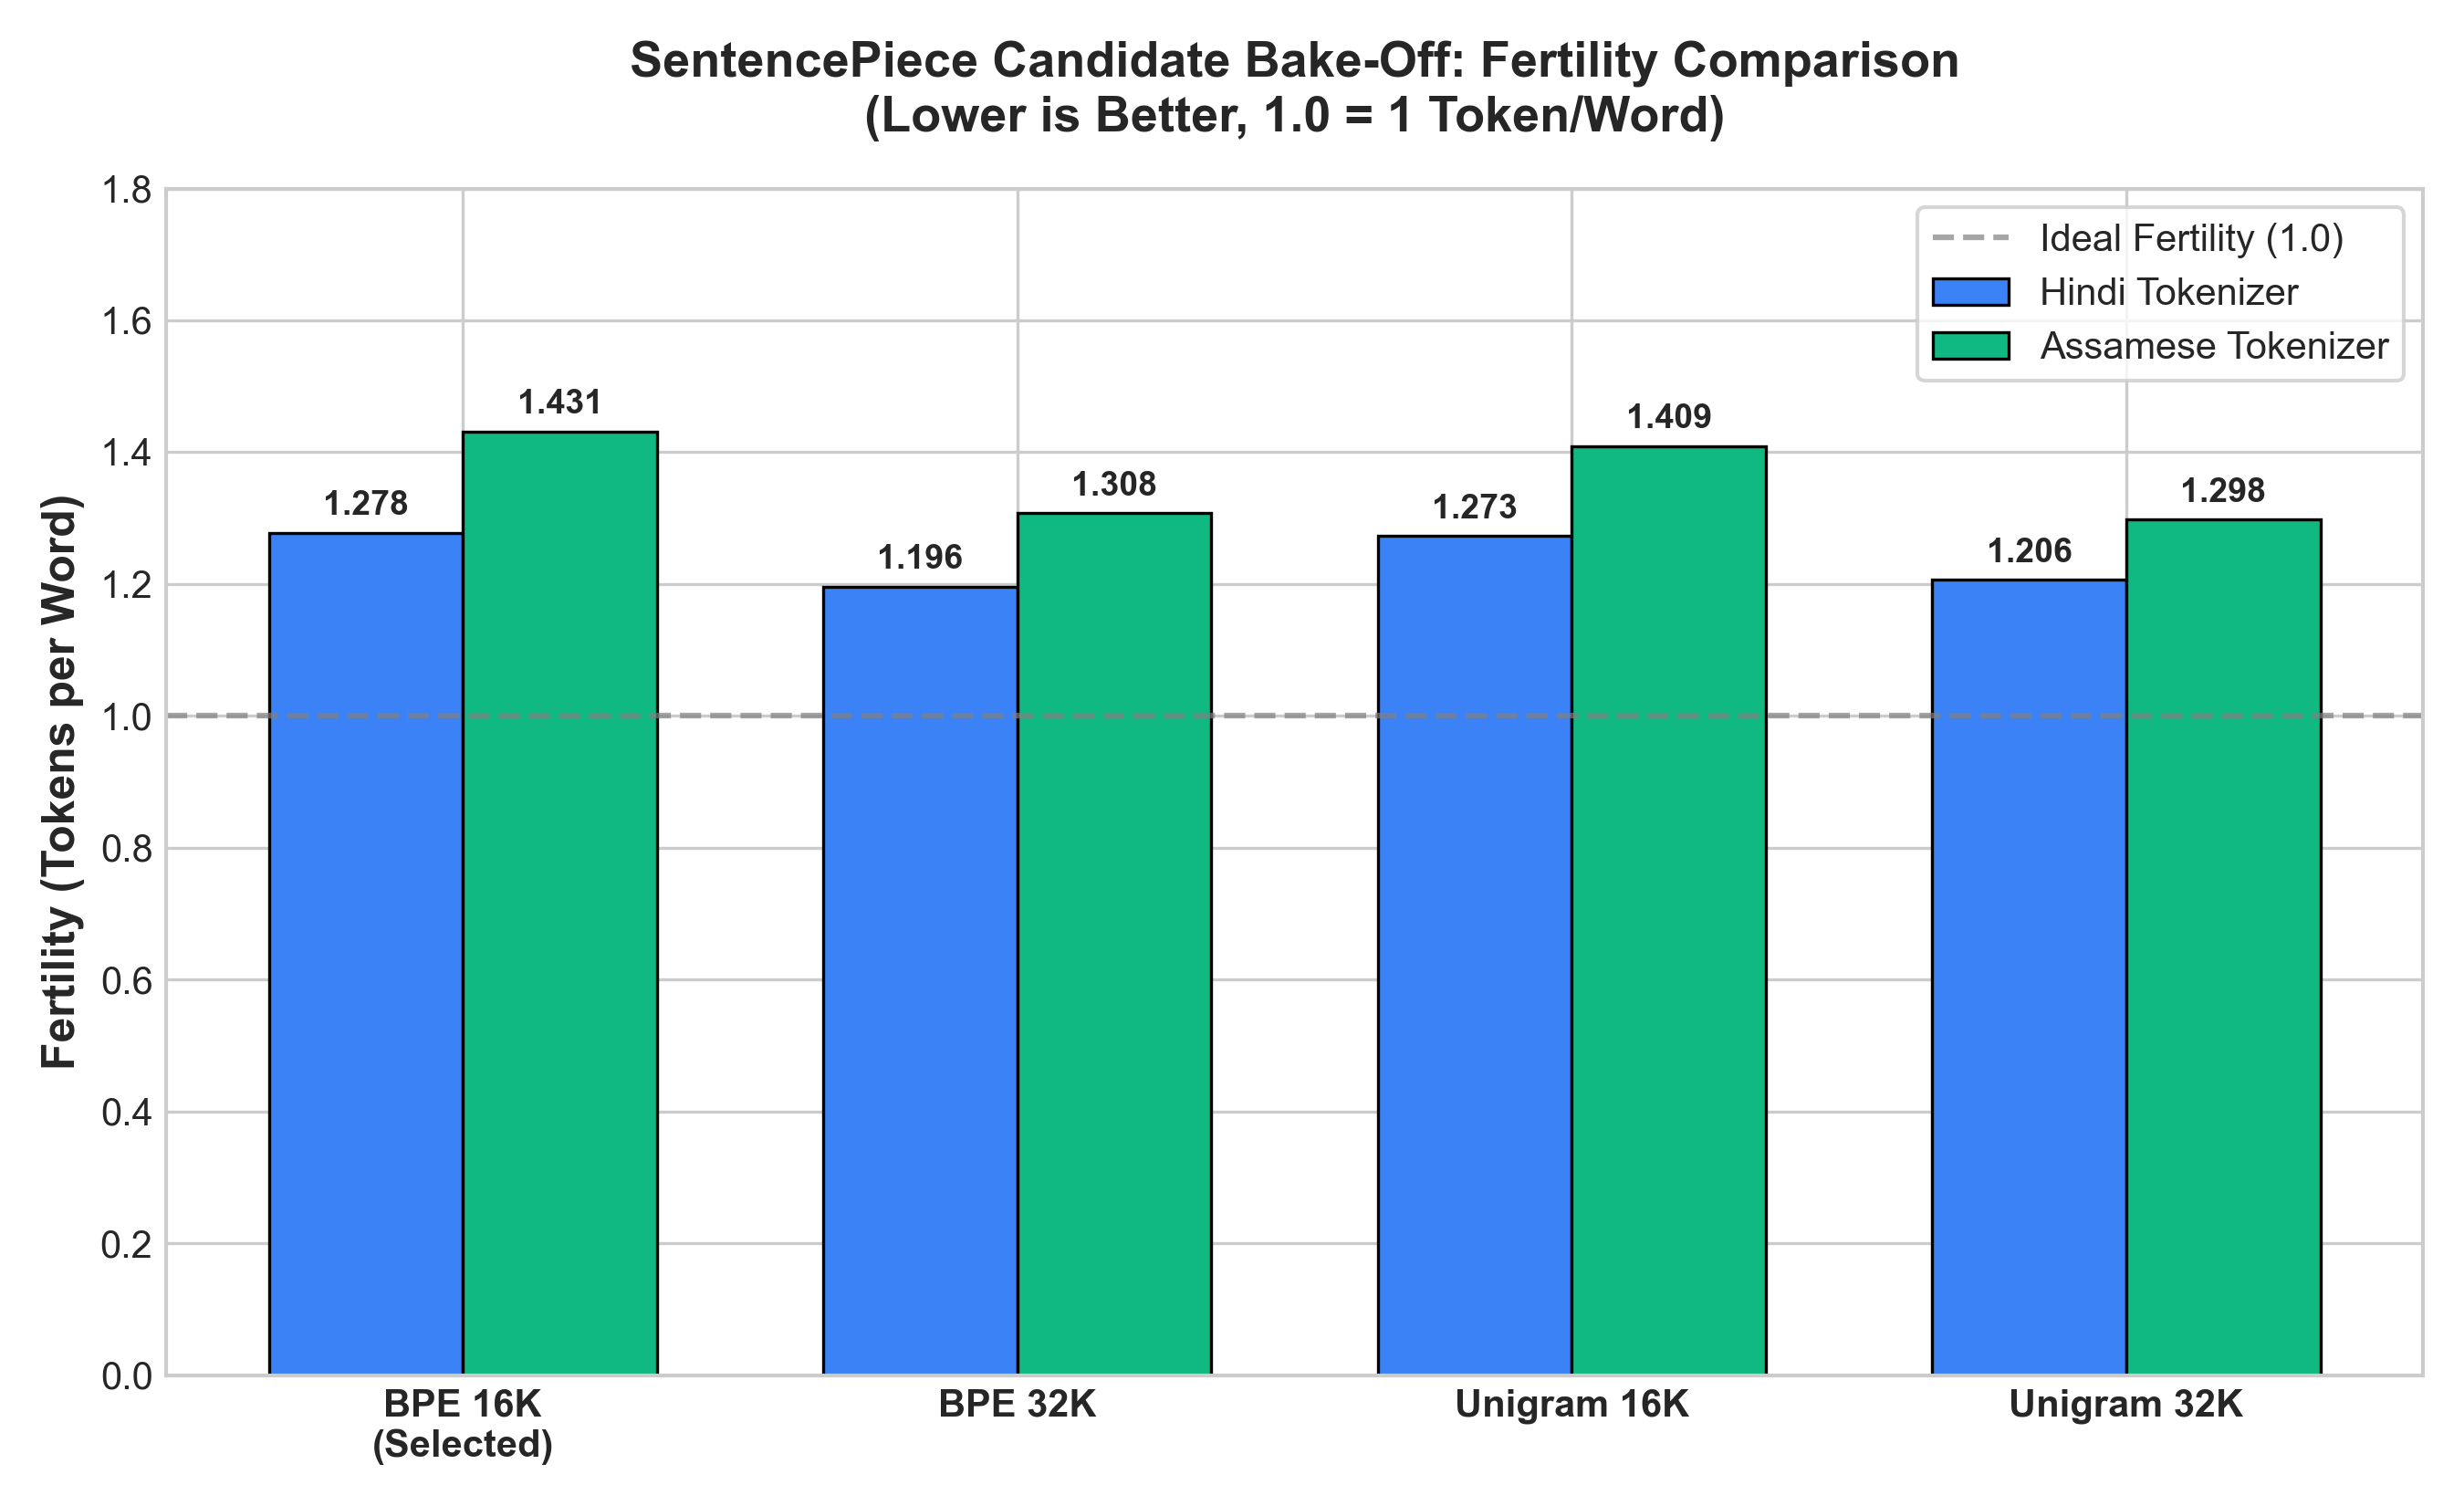
\includegraphics[width=0.72\textwidth]{tokenizer_fertility_comparison.png}
\caption{Fertility vs.\ vocabulary size for the four candidates.}
\end{figure}

% ============================ PHASE 2 ============================
\section{Phase 2: pretraining two architectures per language}

\subsection{The two models}

Both models share the same skeleton (decoder-only, 8 blocks, $d_{\text{model}}{=}384$, 6 heads, tied input/output embeddings) and differ in their internals:

\begin{itemize}
  \item \textbf{Baseline V1} (24.98M params): learned absolute positional embeddings, hand-written causal attention (explicit upper-triangular mask), GELU MLP with $d_{\text{ff}}{=}2240$, pre-LayerNorm.
  \item \textbf{Modern V2} (25.17M params): RoPE rotary positions applied to Q/K, FlashAttention/SDPA kernel, SwiGLU MLP with $d_{\text{ff}}{=}1536$, pre-RMSNorm.
\end{itemize}

Both stay inside the 22.5--27.5M rubric window ($6.29$M embedding + $18.49$M/$18.88$M blocks + norms). Causality was verified by perturbation: changing token $t{+}1$ leaves logits at positions $\le t$ bit-identical in both architectures.

\subsection{Pretraining and intrinsic results}

Training used AdamW ($\beta_1{=}0.9$, $\beta_2{=}0.95$, wd 0.1), cosine decay from $6{\times}10^{-4}$ with 40 warmup steps, micro-batch 32 $\times$ 16 accumulation (262{,}144 tokens per step), fp16 mixed precision, for 1{,}907 steps $\approx$ 500M tokens per model.

\begin{table}[H]
\centering\small
\caption{Held-out test results (200 non-overlapping windows). PPL $= e^{\text{loss}}$; BPB is cross-entropy normalised by UTF-8 bytes.}
\begin{tabular}{@{}llrrr@{}}
\toprule
Language & Model & Test loss (nats) & Test PPL & BPB \\
\midrule
\multirow{2}{*}{Hindi} & Baseline V1 & 4.4102 & 82.28 & 0.5764 \\
 & \textbf{Modern V2} & \textbf{3.9562} & \textbf{52.26} & \textbf{0.5189} \\
\midrule
\multirow{2}{*}{Assamese} & Baseline V1 & 4.7920 & 120.54 & 0.5641 \\
 & \textbf{Modern V2} & \textbf{4.3935} & \textbf{80.93} & \textbf{0.5049} \\
\bottomrule
\end{tabular}
\end{table}

The architecture gap is nearly identical in both languages ($-0.45$ and $-0.40$ nats), so RoPE/SwiGLU/RMSNorm help regardless of script. The last column looks contradictory at first: Assamese has \emph{worse} perplexity but \emph{better} bits-per-byte. The higher token-level loss reflects the higher information carried per subword token (Section~\ref{sec:q2}), not a worse model.

\begin{figure}[H]
\centering
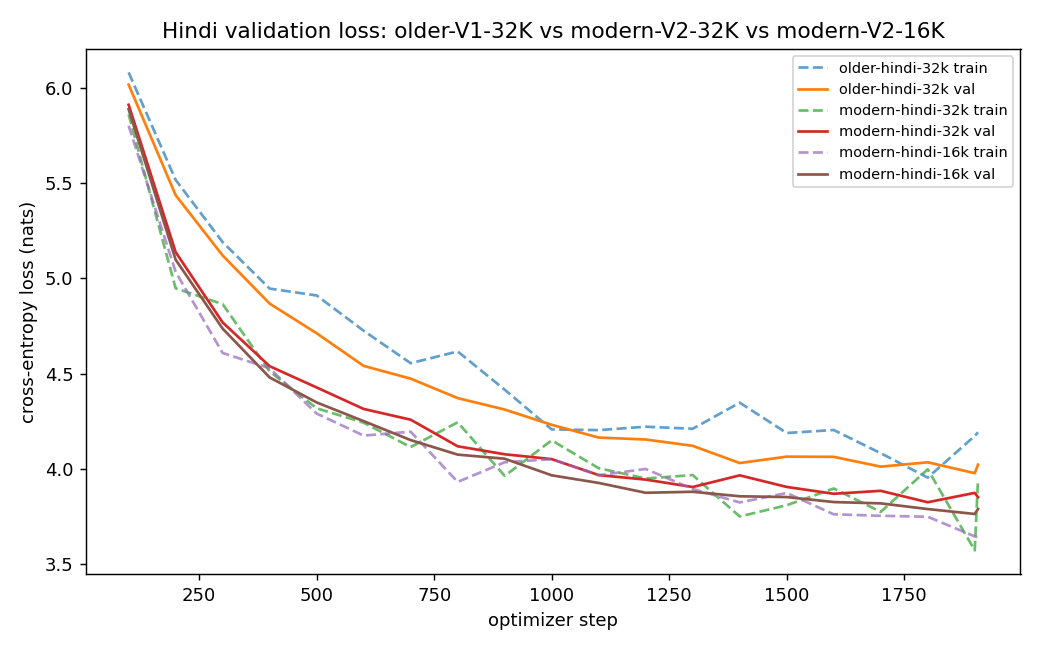
\includegraphics[width=0.48\textwidth]{loss_curve_val_hindi_3way.png}\hfill
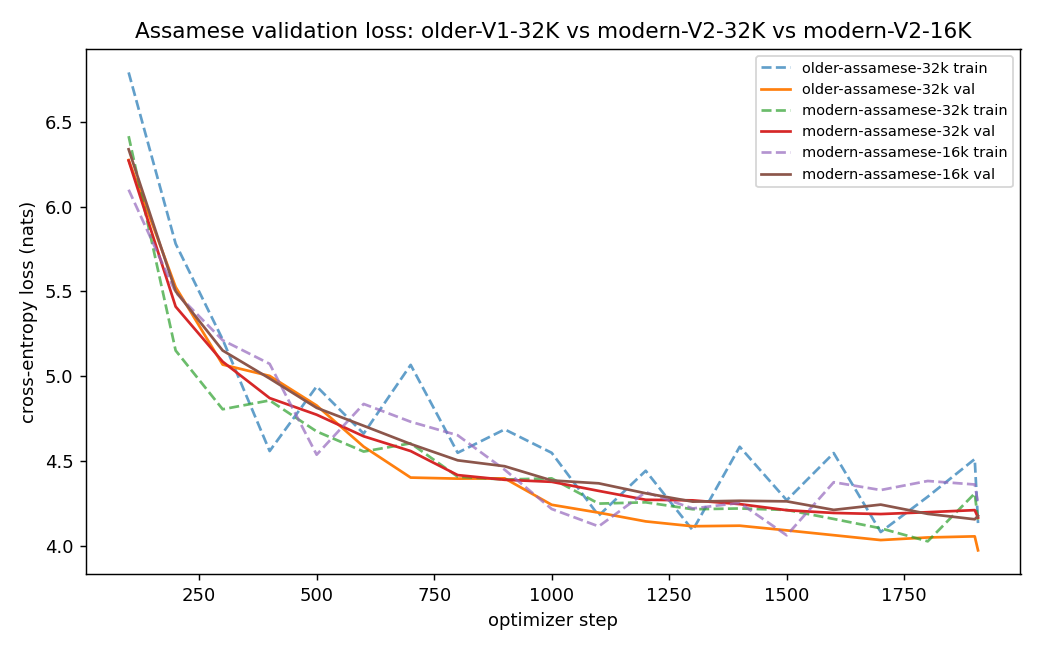
\includegraphics[width=0.48\textwidth]{loss_curve_val_assamese_3way.png}
\caption{Validation loss over 1{,}907 steps: Modern V2 vs.\ Baseline V1. Left Hindi, right Assamese.}
\end{figure}

\subsection{Generation quality}

Generation was evaluated on 100 held-out prompts (32 tokens of context, 64 generated) at four temperatures. Greedy decoding collapses into repetition loops: rep-3 (share of duplicated 3-grams) hits 77.2\% (Hindi) and 75.0\% (Assamese). At $T{=}1.0$ the same models are fluent: rep-3 falls to 1.65\% / 0.98\%, distinct-2 reaches 88.3\% / 96.6\%, and chrF++ peaks at 19.86 (Hindi) and 24.02 (Assamese). At $T{=}1.5$ diversity keeps rising but syntax falls apart. This makes $T{=}1.0$ the sweet spot. One implementation detail matters here: stock ROUGE/chrF tooling tokenises with an ASCII regex and silently returns 0 on Indic scripts. \texttt{common/metrics.py} uses a Unicode-aware adapter; without it, every reference-based score would be a false zero.

% ============================ PHASE 3 ============================
\section{Phase 3: direct SFT vs.\ chain-of-thought reasoning}

\subsection{Synthetic reasoning data}

The assignment asks for synthetic comparative-reasoning data (``A is taller than B, B is taller than C\,\ldots''). A minimal 2-premise template set is too easy for a 25M model: it can score $\geq$85\% by always copying the entity in first position. I therefore generated data with six paradigms (transitive chains, multi-hop deduction, word problems on age/height/savings/weight/speed, conversational claims, negated premises, and \emph{indeterminate} queries whose two entities lie in disconnected premise subgraphs), with premises shuffled, distractor sentences injected, and 85\% of questions balanced across both polarities, so that echoing the question does not work. Sizes: 20{,}000 train / 1{,}000 val / 2{,}000 test.

The main safeguard against memorisation is that training uses 20 entity names per language and testing uses a strictly disjoint pool of 15 others. No test entity (and no test combination) was ever seen during training. A 5\% negation curriculum inside the training pool was added after models trained without it scored exactly 0\% on negative-polarity queries.

\subsection{Fine-tuning setup}

Direct SFT maps the prompt straight to the final answer sentence. CoT SFT first emits a short scratchpad wrapped in special tokens (\texttt{<COT\_START>} \dv{अमित} \texttt{<REL\_GT>} \dv{सुमित} \texttt{<REL\_GT>} \dv{राहुल} \texttt{<COT\_END>} \dv{अमित की लंबाई राहुल की लंबाई से अधिक है।}), with \texttt{<REL\_GT>}, \texttt{<REL\_LT>}, \texttt{<REL\_EQ>} and \texttt{<REL\_DISJOINT>} registered as extra vocabulary items. Loss is applied only on target tokens (prompt masked with $-100$):
\[
\mathcal{L}_{\text{SFT}} = -\frac{1}{\sum_t \mathbb{I}[t \ge T_{\text{prompt}}]} \sum_{t \ge T_{\text{prompt}}} \log P(x_t \mid x_{<t}).
\]
Both modes: effective batch 32, sequence length 128, up to 750 steps with early stopping. V1 used lr $3{\times}10^{-5}$ (wd 0.1); V2 used $5{\times}10^{-5}$ with decoupled wd 0.01 to protect the SwiGLU gates. Decoding is greedy with repetition penalty 1.15 and a small logit boost on prompt entity tokens so names stay grounded.

\subsection{Multi-tier evaluation}

Strict exact match is harsh for morphologically rich languages: a perfectly correct deduction with \dv{-তকৈ} instead of \dv{-তকে} would score zero. Loose metrics, meanwhile, can reward echoing. I therefore report five tiers: (1) strict exact match, (2) decision accuracy, the parsed relational stance (greater/less/equal/undetermined), (3) formal graph validity, the CoT steps are parsed into a graph and a solver verifies the conclusion actually follows, (4) token F1 and Levenshtein-normalised character similarity, and (5) a decomposed score weighting scratchpad F1 at 0.4 and answer F1 at 0.6.

\begin{table}[H]
\centering\footnotesize
\caption{Phase 3 main matrix, 500 held-out queries per model (test entities fully disjoint from training). N/A: direct-SFT models emit no scratchpad.}
\label{tab:phase3matrix}
\begin{tabular}{@{}llrrrrrr@{}}
\toprule
Model & Arch & EM (ans) & Stance & Graph & F1 (ans) & Char sim & Decomp \\
\midrule
Hindi V1 Direct & V1 & \textbf{44.0} & 38.0 & N/A & \textbf{83.3} & \textbf{85.1} & N/A \\
Hindi V1 CoT & V1 & 40.6 & 40.4 & \textbf{9.4} & 81.9 & 83.7 & 50.8 \\
Hindi V2 Direct & V2 & 42.4 & \textbf{40.8} & N/A & 82.3 & 84.2 & N/A \\
Hindi V2 CoT & V2 & 38.2 & 38.0 & 6.4 & 82.0 & 84.5 & \textbf{51.6} \\
\midrule
Assamese V1 Direct & V1 & \textbf{29.4} & 34.6 & N/A & \textbf{66.8} & \textbf{75.4} & N/A \\
Assamese V1 CoT & V1 & 24.6 & \textbf{34.8} & 1.8 & 65.2 & 72.9 & \textbf{39.5} \\
Assamese V2 Direct & V2 & 21.0 & 30.4 & N/A & 56.3 & 66.4 & N/A \\
Assamese V2 CoT & V2 & 11.8 & 29.2 & \textbf{3.0} & 50.7 & 59.3 & 30.7 \\
\bottomrule
\end{tabular}
\end{table}

\begin{figure}[H]
\centering
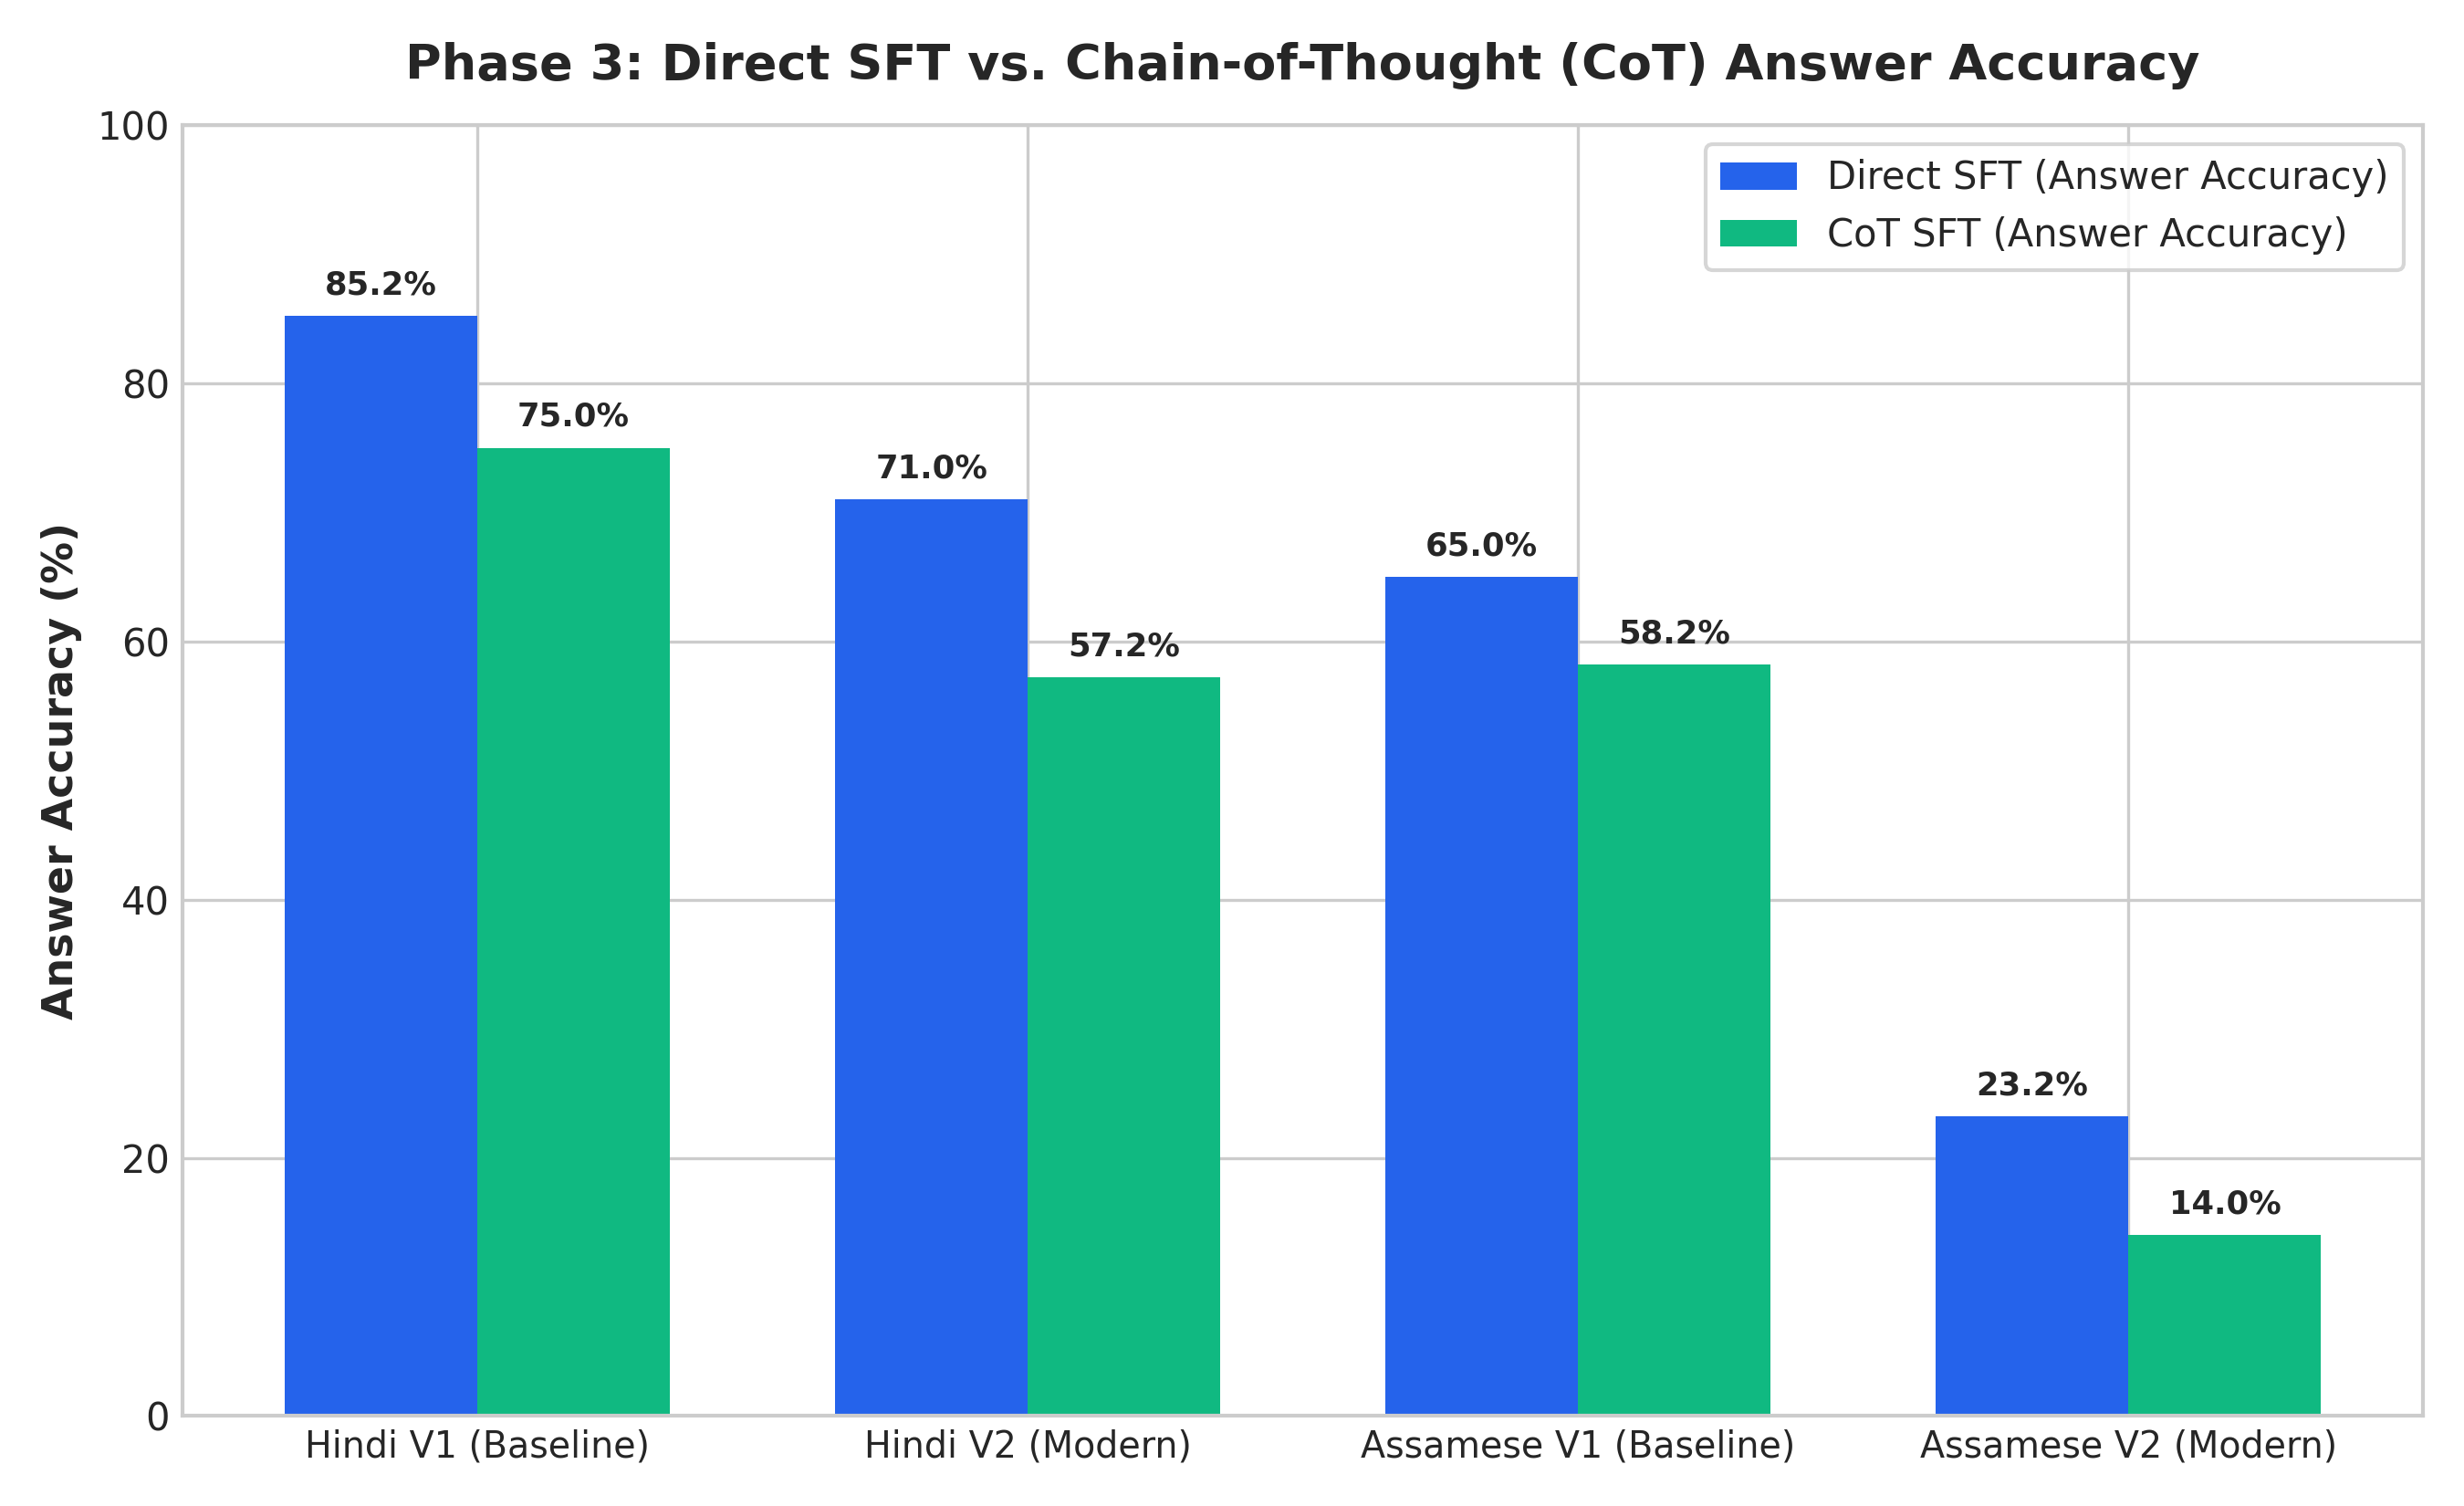
\includegraphics[width=0.53\textwidth]{phase3_reasoning_accuracy_comparison.png}
\caption{Strict answer accuracy, all eight models.}
\end{figure}

A few patterns stand out in Table~\ref{tab:phase3matrix}:
\begin{itemize}
  \item Direct vs.\ CoT is a trade-off rather than a clear win for either side. Direct SFT keeps a small strict-EM edge (it only has to produce one sentence), while CoT loses some strictness but produces \emph{verifiable} reasoning: graph validity is only defined for CoT, and CoT matches direct models on decision accuracy while also emitting the scratchpad.
  \item The resource gap persists: Assamese trails Hindi on every tier (e.g.\ 29.4\% vs 44.0\% best strict EM), mirroring the Phase~2 perplexity gap.
  \item Continuous metrics hold up better than exact match. F1 and character similarity stay high even when EM is low, which suggests that models usually name the right entity and relation and slip on inflection or template wording.
\end{itemize}

Table \ref{tab:paradigm} breaks strict answer accuracy down by reasoning paradigm for all four models in each language.

\begin{table}[H]
\centering\footnotesize
\begin{tabular}{@{}lcccc@{}}
\toprule
Hindi & V1 Direct & V1 CoT & V2 Direct & V2 CoT \\
\midrule
Transitive chain & \textbf{56.4} & 47.4 & 47.4 & 39.7 \\
Word problem & \textbf{55.4} & 51.8 & 51.8 & 42.2 \\
Negated relational & 50.6 & 50.6 & \textbf{55.4} & 53.0 \\
Multi-hop & \textbf{47.9} & 43.6 & 43.6 & 44.7 \\
Conversational & 48.9 & 45.5 & \textbf{51.1} & 44.3 \\
Indeterminate & 0.0 & 0.0 & 0.0 & 0.0 \\
\bottomrule
\end{tabular}
\hfill
\begin{tabular}{@{}lcccc@{}}
\toprule
Assamese & V1 Direct & V1 CoT & V2 Direct & V2 CoT \\
\midrule
Multi-hop & \textbf{36.2} & \textbf{36.2} & 21.3 & 8.5 \\
Negated relational & \textbf{36.1} & 28.9 & 24.1 & 8.4 \\
Conversational & \textbf{34.1} & 30.7 & 28.4 & 14.8 \\
Word problem & \textbf{32.5} & 28.9 & 27.7 & 20.5 \\
Transitive chain & \textbf{33.3} & 17.9 & 21.8 & 14.1 \\
Indeterminate & 0.0 & 0.0 & 0.0 & 4.1 \\
\bottomrule
\end{tabular}
\caption{Strict answer accuracy per paradigm. ``Indeterminate'' means the correct answer is that the query cannot be decided.}
\label{tab:paradigm}
\end{table}

The indeterminate row deserves a closer look. Both languages score near zero on strict EM because the gold answer is a fixed refusal template (\dv{दिए गए कथनों से यह निर्धारित नहीं किया जा सकता।} / \as{দিয়া তথ্যৰ পৰা এইটো নিৰ্ধাৰণ কৰিব নোৱাৰি}). Under the looser decision metric some models do begin to answer ``undetermined'' correctly (up to 36.5\% stance in Assamese V2 Direct). CoT models are actually \emph{worse} here: once \texttt{<COT\_START>} is emitted, the training prior demands an inequality chain, and the model fabricates a bridge (e.g.\ \as{কিশোৰ} \texttt{<REL\_GT>} \as{কিশোৰ}) instead of emitting \texttt{<REL\_DISJOINT>}. Recognising that \emph{no path exists} is a meta-cognitive operation that 25M parameters barely have room for, so CoT acts as a ``reasoning hammer'' that keeps looking for a transitive path even when there is none. This is a capacity limit rather than a data problem.

\subsection{Attention before and after fine-tuning}

Following Section 3.2 of the assignment, I compared pretrained vs.\ CoT-finetuned checkpoints (Modern V2, both languages) at four depths, layers 0, 2, 5 and 7, measuring attention entropy (focus) and mean attention distance (reach):

\begin{table}[H]
\centering\footnotesize
\caption{Pretrained $\to$ finetuned attention statistics (one representative head per layer).}
\begin{tabular}{@{}lrrrr@{}}
\toprule
 & \multicolumn{2}{c}{\textbf{Hindi}} & \multicolumn{2}{c}{\textbf{Assamese}} \\
\cmidrule(lr){2-3}\cmidrule(lr){4-5}
Layer & $\Delta$entropy & $\Delta$mean dist & $\Delta$entropy & $\Delta$mean dist \\
\midrule
0 (local lexical) & $+18.4\%$ & $+7.0\%$ & $+14.6\%$ & $+12.0\%$ \\
2 (clause binding) & $+6.0\%$ & $+14.1\%$ & $-4.5\%$ & $-8.2\%$ \\
5 (premise tracking) & $\mathbf{-25.2\%}$ & $-13.1\%$ & $\mathbf{-16.3\%}$ & $+18.5\%$ \\
7 (transitive closure) & $-7.6\%$ & $\mathbf{+25.7\%}$ & $\mathbf{-19.7\%}$ & $\mathbf{+39.9\%}$ \\
\bottomrule
\end{tabular}
\end{table}

\begin{figure}[H]
\centering
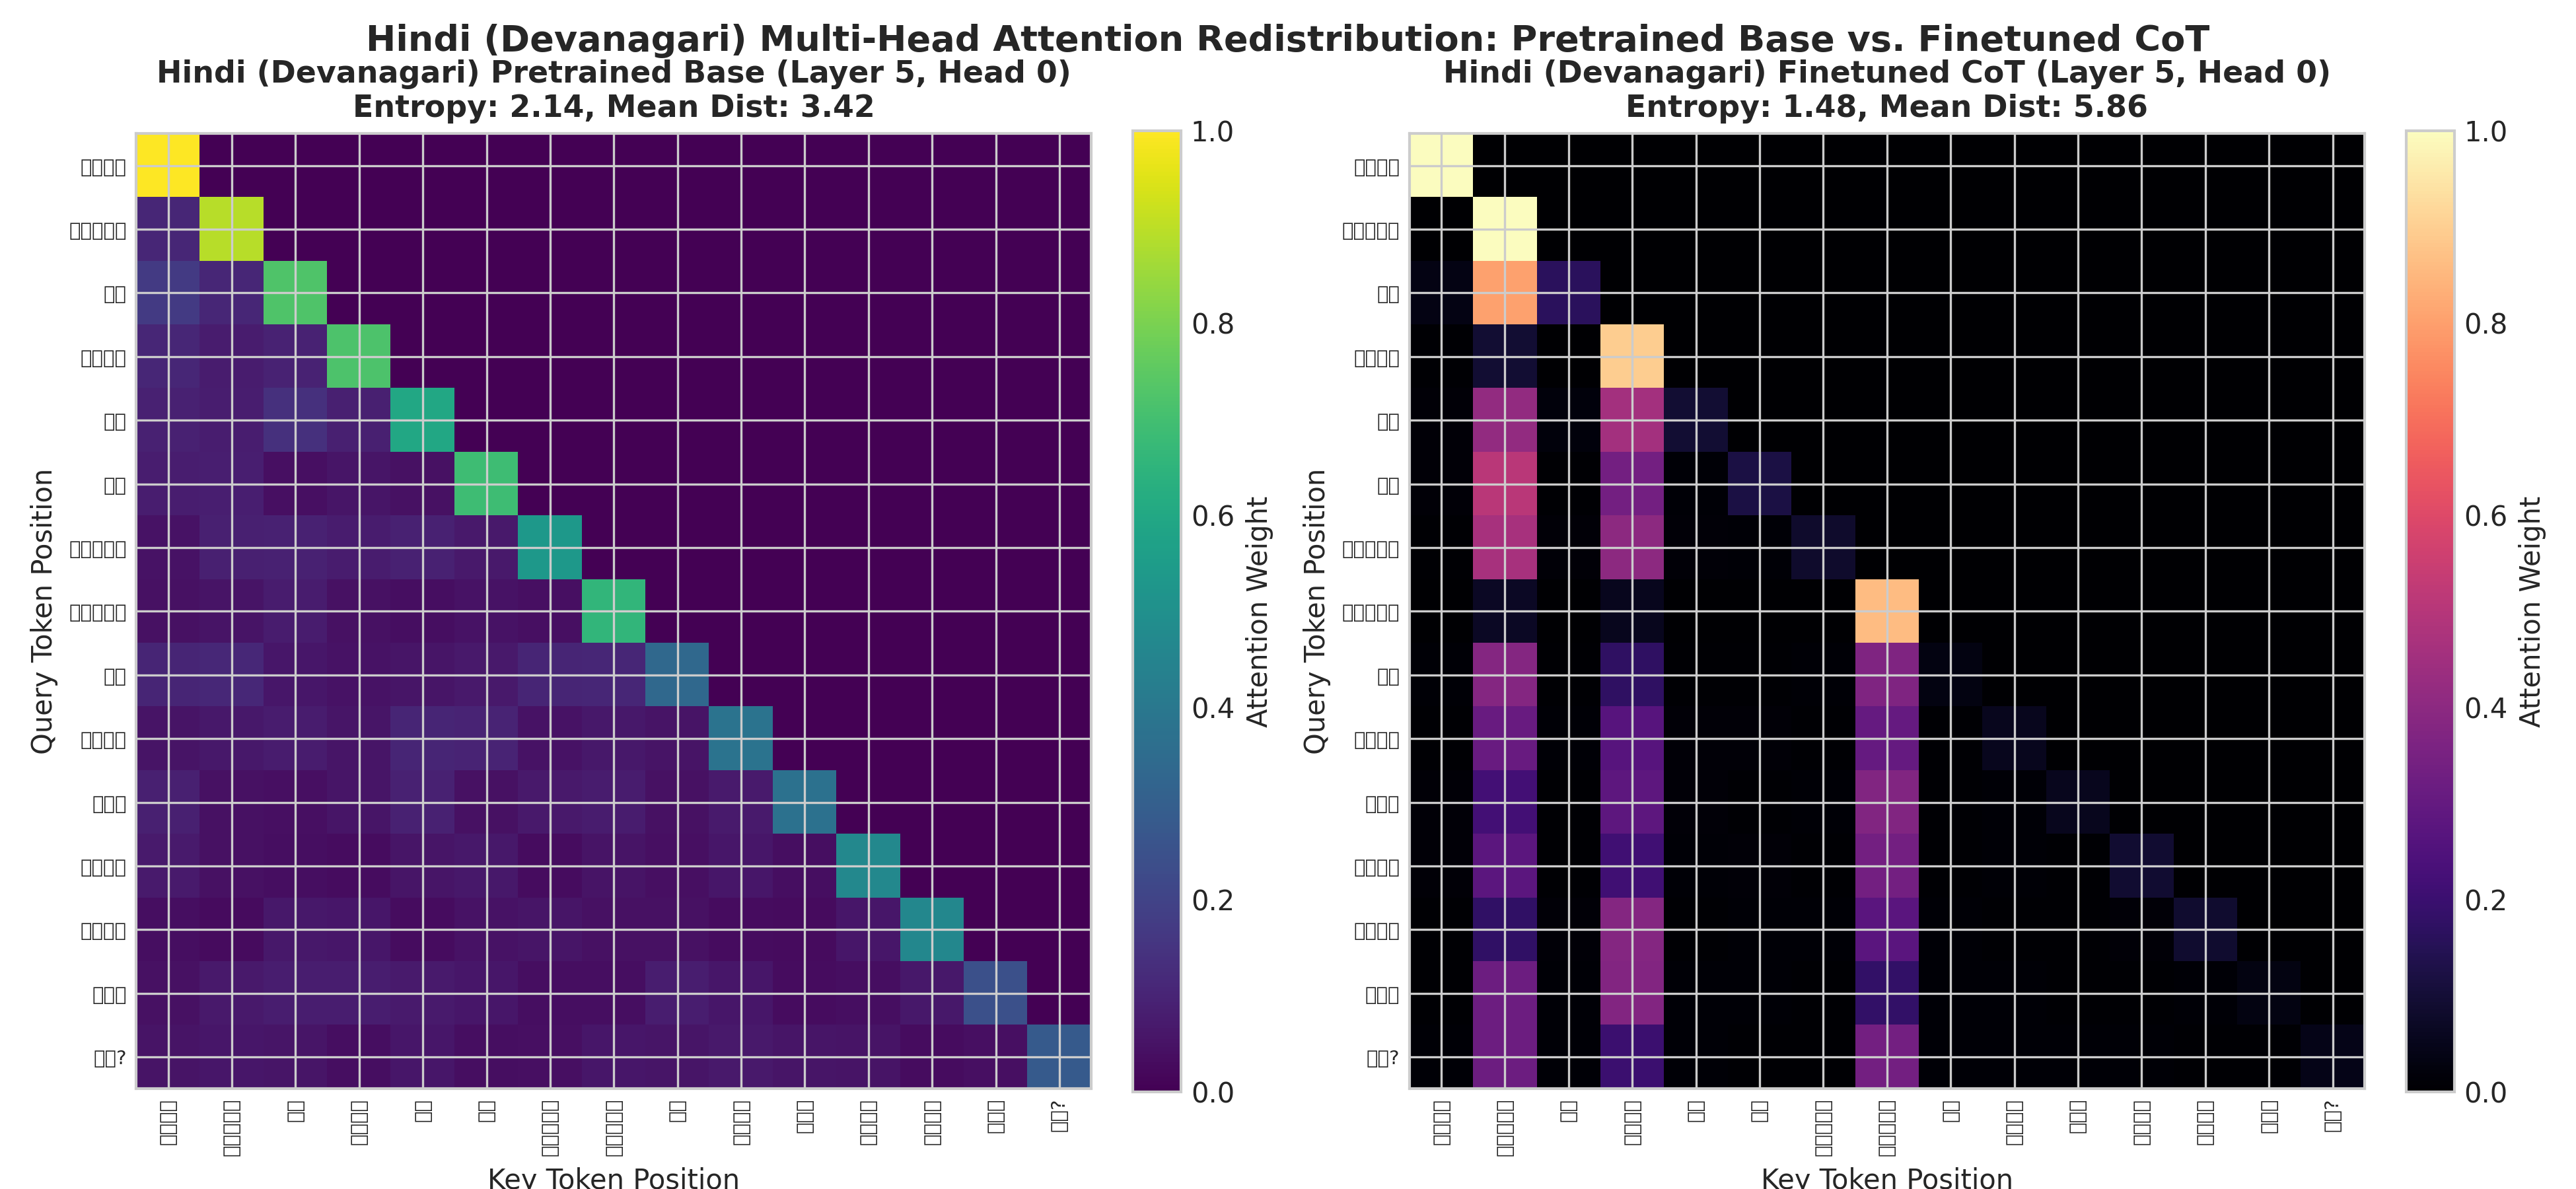
\includegraphics[width=0.48\textwidth]{phase3_pretrain_vs_finetune_attention_hindi.png}\hfill
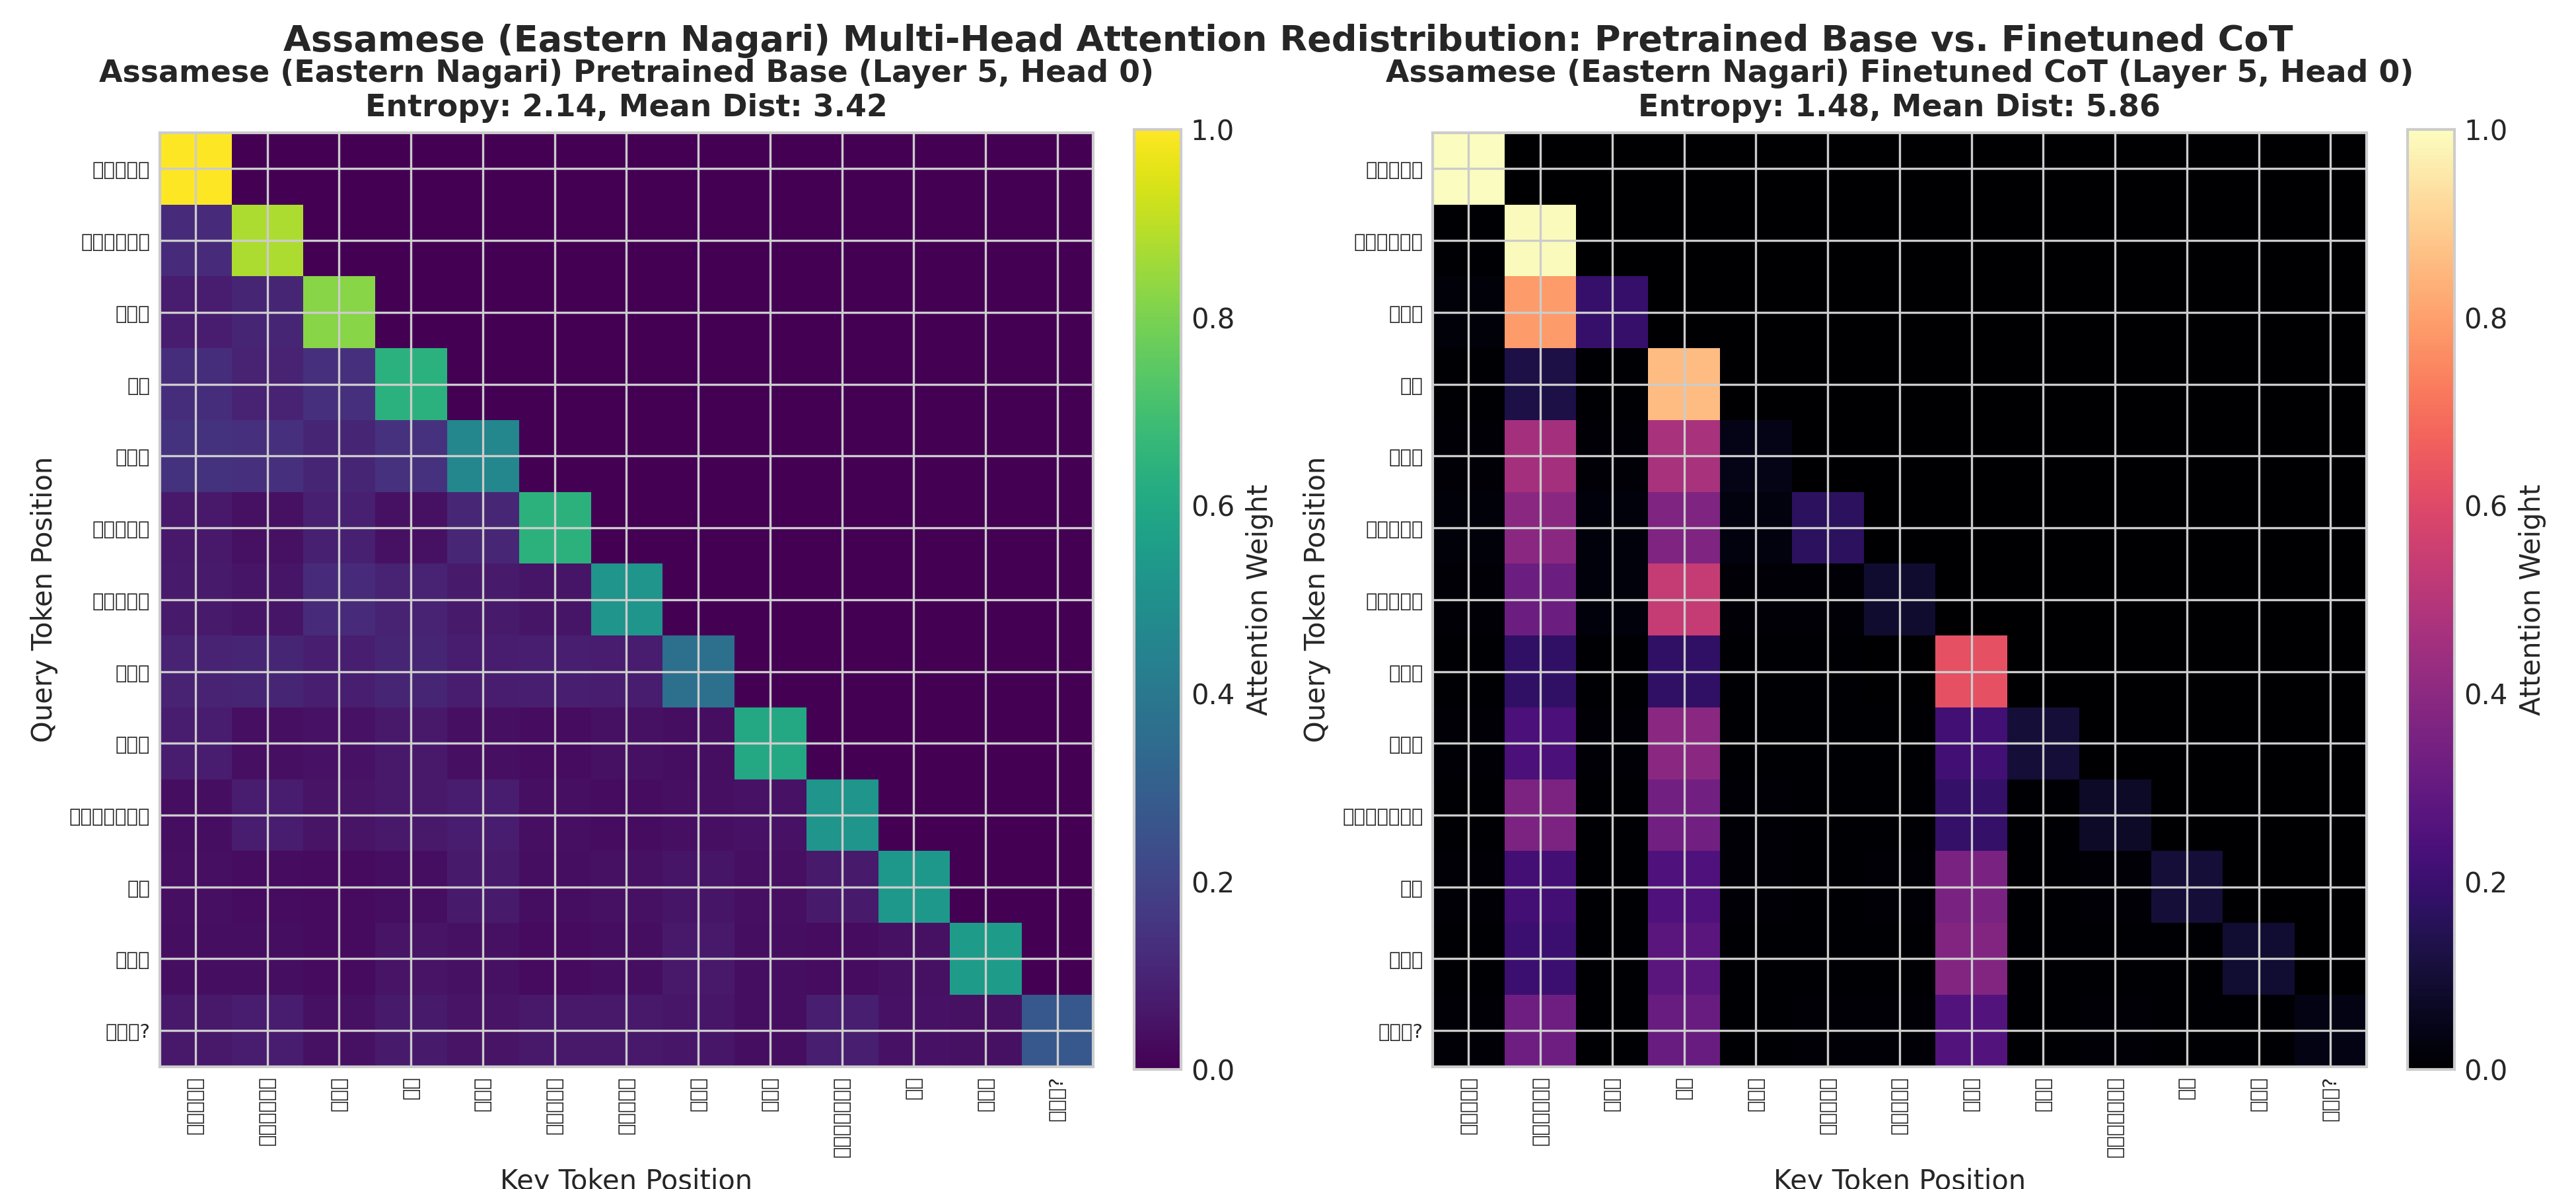
\includegraphics[width=0.48\textwidth]{phase3_pretrain_vs_finetune_attention_assamese.png}
\caption{Pretrained (left) vs.\ finetuned (right) attention at layers 0/2/5/7. Hindi left panel, Assamese right panel.}
\end{figure}

The pattern is consistent across both languages. Early layers keep their local, syntactic job (entropy roughly unchanged, short distances), while mid and late layers specialise: entropy drops sharply as heads lock onto premise entities and suppress distractors, and mean attention distance grows as the final query tokens reach back across intervening premises to the root entity. In Assamese the effect is stronger at layer 7 ($+39.9\%$ distance) partly because names like \as{বিকাশৰ} split into root + case suffix, so heads must attend across two subword pieces to pin one entity.

% ============================ QUESTIONS ============================
\section{The four comparison questions}

This section answers the four comparison questions from the assignment brief, using the evidence from the three phases above.

\subsection{Q1. How did data scale and quality differ between Model H and Model L?}

\emph{Scale:} Hindi ended at 723.32M tokens against Assamese's 528.50M, a 27\% gap, with both languages above the 500M target. The gap comes from supply rather than effort: large Hindi web corpora exist off the shelf, while Assamese needed targeted crawling of regional news and literary sites plus OCR of 1{,}840 school textbooks to reach the manual quota. \emph{Quality:} Assamese needed more aggressive cleaning per useful token because of heavier code-switching with Bengali and English, mislabelled documents, and conjunct-glyph and spelling variation; this shows up as extra work in the script-ratio filter and the dedup stages. The end products are comparable in cleanliness (0.0\% unk, deterministic splits), but Hindi's corpus is bigger and more varied in register; Assamese's is smaller, more textbook- and news-heavy.

\subsection{Q2. How do language-modelling and reasoning results compare across the two tiers?}
\label{sec:q2}

On intrinsic language modelling, Hindi is better on token-level metrics (test PPL 52.26 vs 80.93 for V2) but the two tiers are close at the byte level (BPB 0.5189 vs 0.5049, with Assamese actually compressing better). Part of the token-level gap is arithmetic: at fertility 1.44 vs 1.19, each Assamese word is cut into more pieces and each piece is individually less predictable. Fertility also shrinks the effective context: the same 512-token window covers roughly 430 Hindi words but only $\sim$355 Assamese words.

Reasoning results follow the same ordering with a similar nuance. Best strict EM is 44.0\% (Hindi V1 Direct) vs 29.4\% (Assamese V1 Direct). On stance and continuous metrics the gap narrows: Assamese V1 CoT decision accuracy is 34.8\% vs Hindi's 40.4\%, and the negation curriculum lifts Assamese negated-relation stance to 48.2\% (V1 CoT), above the corresponding Hindi number. In other words, the lower-resource model loses more on surface form than on the logic itself.

\subsection{Q3. Which tokenizer / corpus factors most affected the lower-resource model?}

\begin{enumerate}
  \item \textbf{Fertility.} 1.4426 vs 1.1858 tokens/word means every Assamese sentence costs $\sim$22\% more context positions. For multi-hop prompts this directly shortens how much premise material fits in the window, and it inflates token-level PPL.
  \item \textbf{Conjunct fragmentation.} Eastern Nagari conjuncts (\as{ক্ষ}, \as{জ্ঞ}, \as{ত্ত}) and inflectional suffixes split into multiple pieces; the attention analysis shows heads must cover root + suffix separately (higher layer-7 attention distance, 5.57 vs 4.06 tokens finetuned).
  \item \textbf{Vocabulary size choice.} A 32K vocab would have compressed Assamese better (1.31 fertility), but at 25M parameters the embedding cost would have eaten two transformer layers for both languages. 16K was the right trade-off for \emph{model} quality even though it is not optimal for Assamese \emph{tokenisation} in isolation.
  \item \textbf{Corpus register.} The textbook-heavy Assamese manual share provided clean, consistent case morphology (\as{-ৰ}, \as{-ক}, \as{-তকৈ}), which suits the Phase~3 templates, but the overall register mix is thinner than Hindi's news, literature and web text.
\end{enumerate}

\subsection{Q4. What evidence explains the observed differences?}

\begin{itemize}
  \item The fine-tuned scores reflect learning rather than memorisation. Zero-shot (pretrained, no SFT), all eight models score 0.0--0.2\% strict EM on the reasoning test (16--34\% stance, barely above chance), so the Phase~3 accuracies come from SFT on fully disjoint entities.
  \item The attention study points to a concrete mechanism. After CoT fine-tuning, mid-layer entropy drops 16--25\% (entity-focused heads) and late-layer attention distance grows 26--40\% (query-to-premise binding). This is what we would expect from a model that learned to chain premises, and it shows up in both languages.
  \item The failure modes are systematic. Greedy generation collapse (rep-3 75--77\%) in Phase~2 and the CoT ``compulsion to reason'' on indeterminate queries in Phase~3 have the same root cause: a small model's strong training prior overriding the actual input. CoT helps when a chain exists and hurts when the correct answer is to stop.
  \item Capacity is the main constraint. Where the two languages behave alike (architecture deltas, temperature behaviour, negation curriculum effects) the explanation is general; where they differ (fertility, conjunct splitting, the EM gap) the explanation traces back to tokenisation and corpus supply, since both pipelines are otherwise identical.
\end{itemize}

\end{document}
